\documentclass[12pt]{article}
\usepackage[utf8]{inputenc}
\usepackage{amsmath}
\usepackage{graphicx}
\usepackage{float}
\usepackage[margin=1in]{geometry}
\usepackage{lineno}
\setlength{\parindent}{2em}
\setlength{\parskip}{1em}
\renewcommand{\baselinestretch}{1.2}
\newcommand\dbyd[2]{\frac{\mathrm d{#1}}{\mathrm d{#2}}}
\newcommand{\R}{\mathcal{R}}
\usepackage{color}
\newcommand{\david}[1]{\textcolor{blue}{$\langle${\slshape{\bfseries David:} #1 }$\rangle$}}
\usepackage[colorlinks=true,linkcolor=blue]{hyperref}
\newcommand{\pmV}{p_{V}}
\newcommand{\pmI}{p_{I}}

\title{Intentional infect susceptible with disease induced mortality rate}

\begin{document}
\linenumbers
\maketitle

\section{Introduction}

We also have to consider intentionally infect susceptible individuals with disease induced mortality rate being considered.

\section{System of differential equations}

Since we have to consider disease induced mortality rate, we need to adjust our model by adding extra terms representing mortality rate.

The following assumptions are used:

\begin{itemize}
\item Birth and natural death rate are the same.
\item The latent period is short enough to be ignored.
\item All susceptible individuals are equally likely to be infected, and all infected individuals are equally infectious.
\end{itemize}

\begin{subequations}\label{1}
\begin{align}
\dbyd{S}{t}&=\mu- \beta S(V+I)-rS-\mu S \,,\\
\dbyd{V}{t}&=\beta SV+rS-\gamma V -\mu V\,,\\
\dbyd{I}{t}&=\beta SI-\gamma I -\mu I\,,\\
\dbyd{M}{t}&=\pmV\gamma V+\pmI\gamma I\,,\\
\dbyd{R}{t}&=(1-\pmV)\gamma V+(1-\pmI)\gamma I-\mu R\,,
\end{align}
\end{subequations}

Where $\beta$ is transmission rate, $\gamma$ is recovery rate, $\mu$ is the \emph{per capita} rate of birth and death, $r$ is the rate of intensional infection on susceptible individuals.

We non-dimensionalize \autoref{1} by scaling time, by
\begin{equation}
\tau=(\gamma+\mu)t \,,
\end{equation}

As the result, we obtain,

\begin{subequations}\label{eq:base}
\begin{align}
\dbyd{S}{\tau}&=\epsilon-\eta S-\R_0 S(V+I)-\epsilon S\,, \label{3a}\\
\dbyd{V}{\tau}&=\R_0 SV+\eta S-V\,, \label{3b}\\
\dbyd{I}{\tau}&=\R_0 SI-I\,, \label{3c}\\
\dbyd{M}{\tau}&=\pmV(1-\epsilon) V+\pmI(1-\epsilon) I\,,\\
\dbyd{R}{\tau}&=(1-\pmV)(1-\epsilon) V+(1-\pmI)(1-\epsilon) I-\epsilon R\,,
\end{align}
\end{subequations}

Where $\epsilon=\frac{\mu}{\gamma+\mu}$, $\R_0=\frac{\beta}{\gamma+\mu}$, $\eta=\frac{r}{\gamma+\mu}$

\section{Equilibria}

To solve for all equilibria for this system of ODEs, we let \autoref{3a}, \autoref{3b} and \autoref{3c} equal to 0 and solve for solutions.

By letting \autoref{3c} equal to 0, we have either $S=\frac{1}{\R_0}$, $I=0$ or both. For the case where $S=\frac{1}{\R_0}$, \autoref{3b} returns,
\begin{equation}
\dbyd{V}{\tau}=\eta S =0\,,
\end{equation}
Since we consider a non-zero rate of intentional infection, we could conclude that $I=0$.

Therefore, by substituting back into \autoref{3a} and \autoref{3b}, we get

\begin{subequations}\label{eq:EE}
\begin{align}
\hat{S} &= \frac{1}{\R_0}-\frac{2\eta}{\R_0(-(\eta+\epsilon-\epsilon\R_0)+\sqrt{(\eta+\epsilon-\epsilon\R_0)^2+4\R_0\epsilon \eta}+2\eta)}\,, \label{eq:Shat}\\
\hat{V} &= \frac{-(\eta+\epsilon-\epsilon\R_0)+\sqrt{(\eta+\epsilon-\epsilon\R_0)^2+4\R_0\epsilon \eta}}{2\R_0}\,, \label{eq:Vhat}\\
\hat{I} &= 0\,,
\end{align}
\end{subequations}

Clearly $\hat{V}$ is non-zero, therefore this equilibrium is not a disease free equilibrium. It follows that it is the endemic equilibrium.

\section{Stability of Endemic Equilibrium}

The Jacobian matrix of this system is,
\begin{equation}
\mathcal{J} =
\begin{bmatrix}
    \ -\eta-\R_0 (V+I)-\epsilon       & -\R_0 S     &-\R_0 S\\
    \ \R_0 V+\eta       & \R_0 S-1    &0\\
    \ \R_0 I       &0     &\R_0 S-1\\
\end{bmatrix}\,.
\end{equation}

Eigenvalues of Jacobian are ,
\begin{subequations}
\begin{align}
\lambda_1&=-1+\R_0 S \label{eq:lambda1}\\
\lambda_2&=\frac{-1+\R_0 S-\eta-\epsilon-\R_0 V+\sqrt{(-1+\R_0 S-\eta-\epsilon-\R_0 V)^2-4(\eta+\R_0 V+\epsilon-\R_0 S\epsilon)}}{2}\\
\lambda_3&=\frac{-1+\R_0 S-\eta-\epsilon-\R_0 V-\sqrt{(-1+\R_0 S-\eta-\epsilon-\R_0 V)^2-4(\eta+\R_0 V+\epsilon-\R_0 S\epsilon)}}{2}
\end{align}
\end{subequations}

By using \autoref{eq:Shat} and \autoref{eq:lambda1}, we get
\begin{equation}
\Re(\lambda_1)=-1+\R_0 S=-\frac{2\eta}{(-(\eta+\epsilon-\epsilon\R_0)+\sqrt{(\eta+\epsilon-\epsilon\R_0)^2+4\R_0\epsilon \eta}+2\eta)}<0
\end{equation}

To decide the real parts of $\lambda_2$ and $\lambda_3$, we need to determine the sign of the quantity under the square root.

By using \autoref{eq:Shat} again, we have
\begin{equation}
\R_0 S\epsilon<\epsilon\,,
\end{equation}

Therefore
\begin{equation}
(\eta+\R_0 V+\epsilon-\R_0 S\epsilon)>0\,,
\end{equation}

It follows that
\begin{equation}
\sqrt{(-1+\R_0 S-\eta-\epsilon-\R_0 V)^2-4(\eta+\R_0 V+\epsilon-\R_0 S\epsilon)}<|(-1+\R_0 S-\eta-\epsilon-\R_0 V)|\,.
\end{equation}

It follows that we have two cases, if the quantity under square root is negative, then
\begin{equation}
\Re(\lambda_2)=\Re(\lambda_3)=-1+\R_0 S-\eta-\epsilon-\R_0 V<0\,,
\end{equation}

Otherwise, we have
\begin{equation}
\Re(\lambda_3)<\Re(\lambda_2)<0
\end{equation}

We are able to conclude that EE is stable.

\section{Disease Free Equilibrium}
As mentioned above in section 4, disease free equilibrium does not exist for this model.

\section{Disease induced mortality rate at Endemic Equilibrium}

By using \autoref{eq:base} and \autoref{eq:Vhat}, we can find the mortality rate at EE,
\begin{equation}
\dbyd{M}{\tau}=\pmV(1-\epsilon)V=\frac{\pmV(1-\epsilon)\epsilon(\R_0 -1)+ \pmV(1-\epsilon)\epsilon \sqrt{(\R_0-1)^2+4\R_0 p}}{2\R_0}\,, \label{eq:dMdt}
\end{equation}
By plotting it, we obtain the following graph,
\begin{figure}[H]
  \centering
  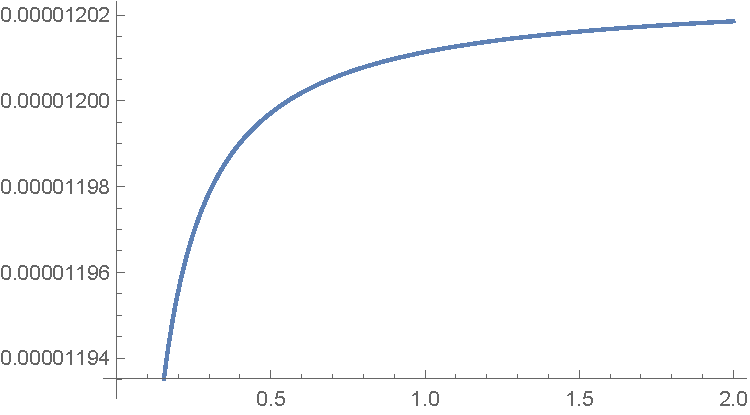
\includegraphics[width=1\textwidth]{Figures/M_at_EE.pdf}
  \caption{$\dbyd{M}{\tau}$ at EE as a function of $\eta$.}
\end{figure}

Again, the magnitude of this mortality rate at EE is way smaller than natural death rate, which has similar result in comparison with newborn model.

The significant difference between two models would be the total mortality count, parameters from \autoref{tab:params} are used to plot the total mortality counts for this model.

\begin{table}[H]
\begin{center}
\caption{Model parameters and smallpox values.}
\label{tab:params}
\smallskip
\begin{tabular}{c|c|r}
{\bfseries Symbol} & {\bfseries Meaning} & {\bfseries Value} \\\hline
$\mu$ & Natural \emph{per capita} death rate & $\frac{1}{50*365}$ per day \\
$\gamma$ & Recovery rate & $\frac{1}{22}$ per day \\
$\R_0$ & Basic reproductive number & 4.5
\end{tabular}
\end{center}
\end{table}

\begin{figure}[H]
  \centering
  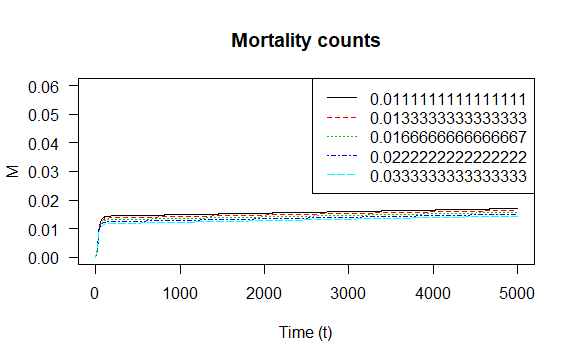
\includegraphics[width=1\textwidth]{Figures/Total_mortality_sus.png}
  \caption{$\dbyd{M}{\tau}$ at EE as a function of $p$.}
\label{fig:dMdt}
\end{figure}

From the scale of the graph, the total mortality count is much lower for this model in comparison with newborn model, this is also why each solution in the figure above has an incline.

\end{document}
